\documentclass[12pt]{article}
\author{Rien Maertens}
\title{GPGPU Project}
\date{11 mei 2016}
\usepackage[dutch]{babel}
\usepackage[utf8]{inputenc}
\usepackage{pgfplots}
\usepackage{float}
\pgfplotsset{compat=newest}

\begin{document}
\maketitle

\part{Per-pixel Image Filters}

\section*{Ontwerpkeuzes}

De verschillende implementaties van {\tt ImageFilter} hebben een hoop gemeenschappelijke functionaliteit (bijvoorbeeld: RGBA-componenten uit een pixel halen en er terug in steken).
Daarom heb ik een paar gemeenschappelijke functies gemaakt die ik in twee categorieën heb ingedeeld:

\begin{description}
    \item [\tt PixelUtils.h]\hfill \\ 
        Dit zijn hulpfuncties om pixels te manipuleren.
        De belangrijkste methodes zijn {\tt getColorData} en {\tt toPixel}.
        Deze gaan door middel van bitoperaties de RGBA-componenten uit een pixel halen en er terug in steken.
        De functies hebben het sleutelwoord {\tt restrict(amp,cpu)} in hun declaratie staan zodat ze op de GPU kunnen uitgevoerd worden.\\
        In dit bestand is ook de methode {\tt colorDistance} geïmplementeerd die de afstand tussen twee kleuren berekent.
    \item [\tt FilterUtils.h]\hfill \\
        Dit zijn functies met betrekking tot het uitvoeren van filter.
Mijn eerste idee was om te werken met een abstracte superklasse voor de GPU, voor de CPU en voor iedere verschillende filter.
Zo zou de {\tt ImageFilter\_Desaturate\_GPU} overerven van een GPU-superklasse en een Desaturate-superklasse.
Helaas kunnen functies met {\tt restrict(amp)} niet virtueel zijn of functiepointer aanroepen.\\ Daarom ben ik overgeschakeld naar het gebruik van lambda's die de manipulaties op de RGBA-componenten voor hun rekening nemen.
Deze lambda's worden als argument meegegeven aan de twee functies in dit bestand:
        \begin{itemize}
            \item{\tt process\_per\_pixel\_GPU}:\\ Hier wordt de C++AMP {\tt parallel\_for\_each}-functie gebruikt om de gegeven afbeelding te verwerken door de GPU.
De arrays met pixels worden gelezen en bewerkt door middel van {\tt array\_view}s.
            \item{\tt process\_per\_pixel\_CPU}:\\ Deze functie doet hetzelfde als hierboven, maar de manipulaties vinden plaats op de CPU.
Deze functie heb ik multithreaded gemaakt: er wordt gekeken hoeveel parallelle threads het systeem aan kan en vervolgens wordt het aantal te verwerken pixels gelijk verdeeld over dit aantal threads.
        \end{itemize}
        Momenteel wordt exact dezelfde lambda gebruikt voor de CPU als de GPU van een filter, maar heb ik nog geen manier gevonden om deze duplicatie te vermijden.
Hier kan er dus eventueel nog een verbetering plaats vinden.
\end{description}

\section*{Uitvoeringstijd CPU en GPU}

Om de uitvoeringstijd per functie te vergelijken heb ik gekeken naar de logs die naar de console werden geschreven bij het uitvoeren van elke functie.
Ik heb opgemerkt dat de eerste functie die op de GPU wordt uitgevoerd significant trager is dan de functies die erna worden uitgevoerd (400 i.p.v 15 milliseconden).
Daarom laat ik eerst een filter draaien voor ik de metingen start.
\\ 
\\
Zoals te zien op figuur \ref{fig:pixel} is de uitvoeringstijd van de CPU-filters het grootst.
Het is logisch dat de multithreaded CPU-filter ongeveer vier keer sneller is dan wanneer alles in serie wordt verwerk: het systeem waarop deze metingen werden uitgevoerd heeft namelijk 4 rekenkernen.
We merken op dat de {\tt Greenscreen}-filter het traagst is.
De oorzaak hiervan kan zijn dat er meer stappen moeten worden uitgevoerd per pixel.
\\
\\
De GPU-filter is dan weer ongeveer 5 keer sneller dan de parallelle CPU-filter, een enorme snelheidswinst.
Onderling is het verschil per filter niet zo groot als bij de CPU-filters.
Een mogelijke verklaring hiervan is dat de effectieve verwerkingssnelheid erg klein is in vergelijking met de overhead veroorzaakt door het kopiëren van data tussen de CPU en GPU.

\begin{figure}[H]
    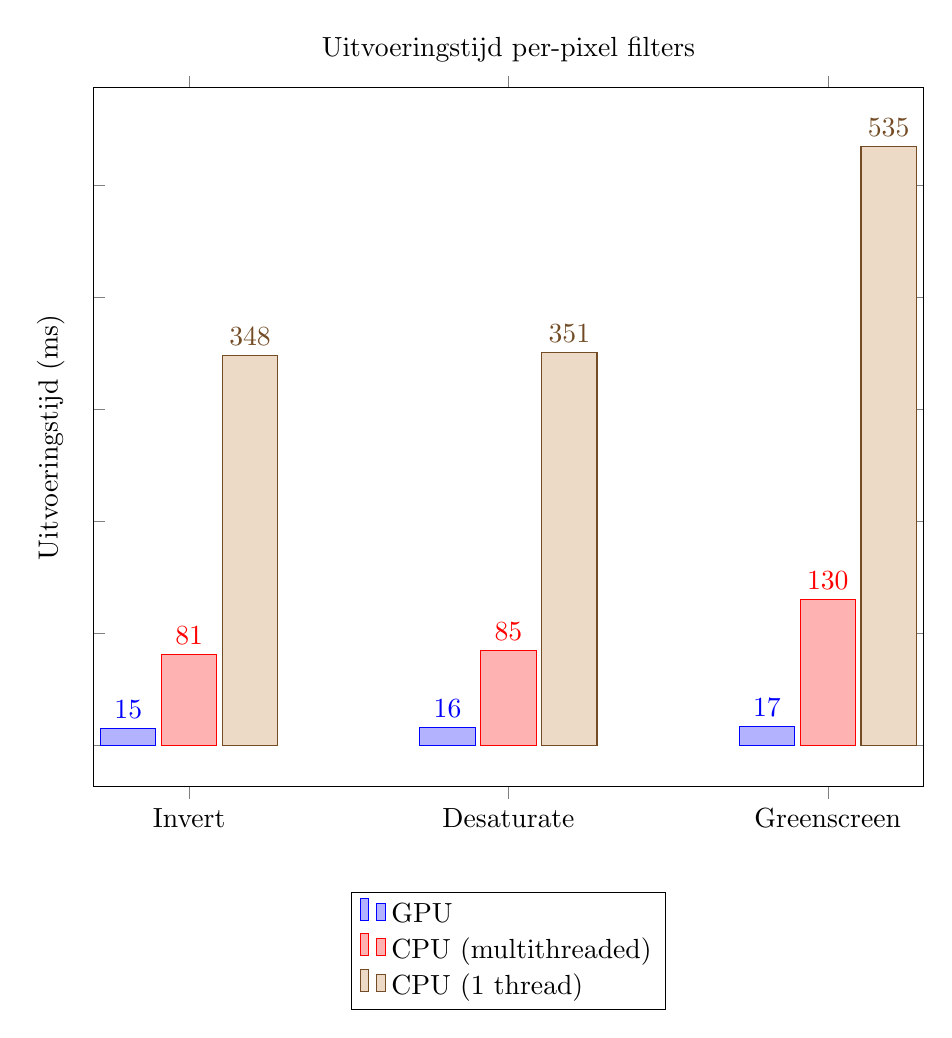
\begin{tikzpicture}
        \begin{axis}[
                title=Uitvoeringstijd per-pixel filters,
                width=\linewidth,
                ylabel=Uitvoeringstijd (ms),
                xtick=data,
                yticklabels={,,},
                enlarge x limits= 0.15, 
                legend style={at={(0.5,-0.15)},
                anchor=north},
                legend cell align=left,
                bar width=20pt,
                symbolic x coords = {Invert, Desaturate, Greenscreen},
                nodes near coords,
            ybar]
            \addplot coordinates {(Invert, 15) (Desaturate, 16) (Greenscreen, 17)};
            \addplot coordinates {(Invert, 81) (Desaturate, 85) (Greenscreen, 130)};
            \addplot coordinates {(Invert, 348) (Desaturate, 351) (Greenscreen, 535)};
            \legend{GPU, CPU (multithreaded), CPU (1 thread)}
        \end{axis}
    \end{tikzpicture}
    \caption{Uitvoeringstijd in milliseconden voor de per-pixel imagefilters.}
    \label{fig:pixel}
\end{figure}

\part{Block-based Image Filters}

\section*{Ontwerpkeuzes}

Voor het tweede deel heb ik twee extra methodes toegevoegd aan de {\tt FilterUtils} die het mogelijk maken om afbeeldingen te verwerken door ze in blokken te splitsen:

\begin{itemize}
    \item {\tt process\_tile\_GPU}: Hier wordt gebruik gemaakt van de tiled extents die worden aangeboden door C++AMP.
Per tile wordt er per kleurcomponent een array aangemaakt met de  
    \item {\tt process\_tile\_CPU}: Deze methode gaat eerst multithreaded de kleurcomponenten extraheren uit de afbeelding.
Vervolgens wordt van de filter gebruik gemaakt om de nieuwe afbeelding te maken.
Deze filter is opnieuw een lambda die wordt meegegeven als argument van de methode.
\end{itemize}

Beide methodes maken gebruik van een nieuwe {\tt WorkBalance}-klasse.
Deze klasse is een hulpmethode om werk (bv.
het aantal te verwerken pixels) te verdelen over een aantal threads.
Deze klasse heeft bovendien een methode {\tt executeParallel} die volgens de berekende verdeling een functie parallel gaat uitvoeren op de CPU.
Ik heb de {\tt process\_per\_pixel\_CPU}-methode van in deel I ook aangepast om deze klasse te gebruiken.
\\
\\
De Median-filter werkt door middel van het sorteren van 9 pixels.
Voor dit sorteren heb ik gebruik gemaakt van een sorteernetwerk: dit is een vaste opeenvolging van vergelijkingen en (indien nodig) verwisselingen.
Ik heb de uitvoeringstijd vergeleken met een insertionsort-implementatie en het sorteernetwerk bleek het snelst te zijn op zowel de GPU als de CPU.

\section*{Uitvoeringstijd CPU en GPU}

Op figuur \ref{fig:block} is het verschil tussen de GPU- en CPU-implementatie te zien.
Hier is de GPU een stuk trager dan bij het vorig deel.
Dit is hoogstwaarschijnlijk het gevolg van de vele (dure) geheugenoperaties die plaats vinden.
Bij de Median-filter valt dit het meest op: er wordt gesorteerd, waardoor een veel verplaatsingen in het geheugen plaats vinden.
Daarnaast kan het ook zijn dat de tilesize die ik gebruik te klein is om een grote snelheidswinst te hebben.



\begin{figure}[H]
    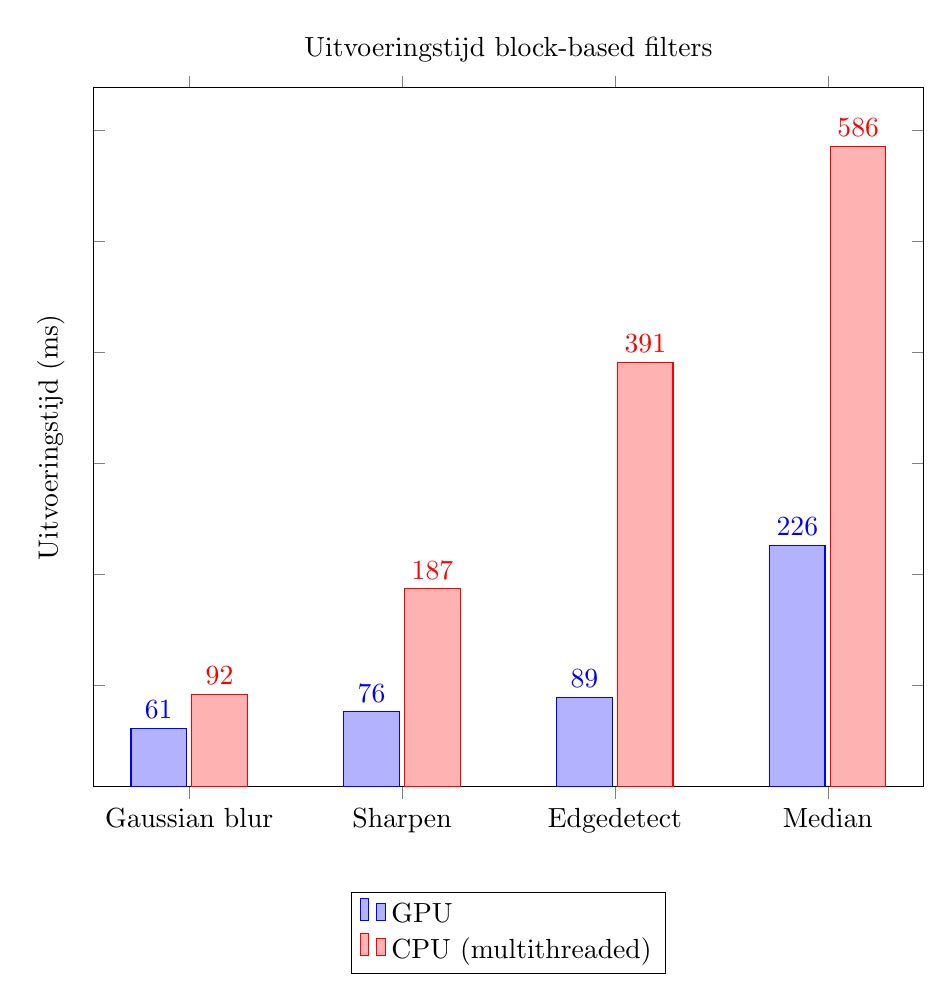
\begin{tikzpicture}
        \begin{axis}[
                title=Uitvoeringstijd block-based filters,
                width=\linewidth,
                ylabel=Uitvoeringstijd (ms),
                xtick=data,
                yticklabels={,,},
                enlarge x limits= 0.15, 
                legend style={at={(0.5,-0.15)},
                anchor=north},
                legend cell align=left,
                bar width=20pt,
                symbolic x coords = {Gaussian blur, Sharpen, Edgedetect, Median},
                nodes near coords,
            ybar]
            \addplot coordinates {(Gaussian blur, 61) (Sharpen, 76) (Edgedetect, 89) (Median, 226)};
            \addplot coordinates {(Gaussian blur, 92) (Sharpen, 187) (Edgedetect, 391) (Median, 586)};
            \legend{GPU, CPU (multithreaded)}
        \end{axis}
    \end{tikzpicture}
    \caption{Uitvoeringstijd in milliseconden voor de block-based imagefilters.}
    \label{fig:block}
\end{figure}

\part{Global Image Filters}

\section*{Ontwerpkeuzes}

Bij dit deel was het niet echt mogelijk om zoals bij de vorige delen te werken met een {\tt process}-methode.
Daarnaast heb ik ook maar één opgave geïmplementeerd dus had het niet veel nut om dit te doen.
\\
De HistogramEqualization-filter werkt op CPU en GPU ongeveer hetzelfde:

\begin{enumerate}
    \item Een frequentietabel van alle v-waardes wordt opgesteld.
    \item De cumulatieve som wordt bepaald.
    \item De nieuwe v-waardes worden berekend.
    \item De v-waardes worden vervangen in de afbeelding.
\end{enumerate}

Enkel stap 2, de cumulatieve som bepalen, wordt niet parallel uitgevoerd.
Via de {\tt amp\_algotithms.h} library heb ik de {\tt scan}-methode even uitgeprobeerd, maar die implementatie was trager dan de seriële implementatie.
Hoogstwaarschijnlijk is de overhead van het kopiëren van data en starten van de threads te groot om een snelheidswinst te verkrijgen.
In de CPU- en GPU-implementatie heb ik er dus voor gekozen om dat stuk serieel te houden.
\\
\\
Om de conversie tussen HSV en RGB te kunnen uittesten heb ik ook een GPU-implementatie voor de Hueshift-filter (deel I) gemaakt.
Deze conversiemethoden staan in {\tt PixelUtils.h}.

\section*{Uitvoeringstijd CPU en GPU}

Zoals te zien op figuur \ref{fig:global} is de GPU-implementatie meer dan 4 keer sneller dan de CPU-implementatie.
Dit is logisch omdat er, net zoals bij de per-pixel filter, niet veel werk moet gebeuren per pixel.
Waar de CPU veel tijd gaat verliezen aan het loopen over alle pixels van de afbeelding kan de GPU veel meer pixels parallel verwerken.

\begin{figure}[H]
    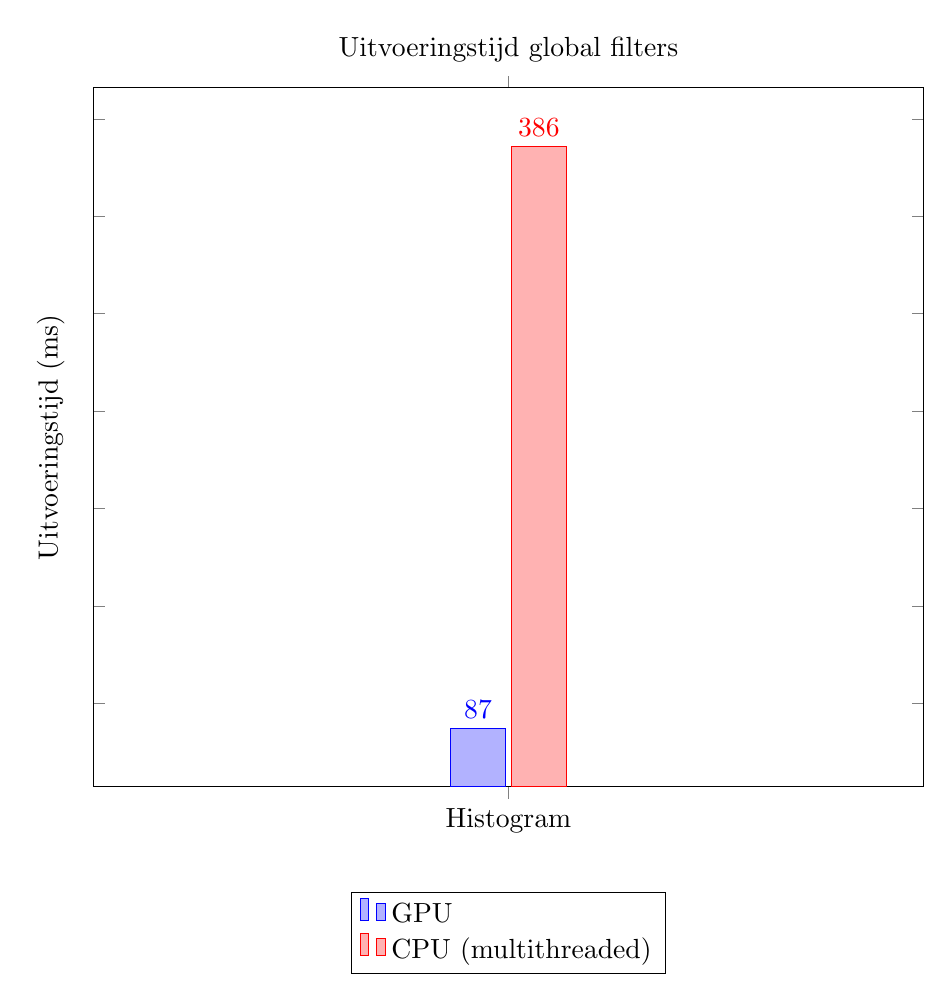
\begin{tikzpicture}
        \begin{axis}[
                title=Uitvoeringstijd global filters,
                width=\linewidth,
                ylabel=Uitvoeringstijd (ms),
                xtick=data,
                yticklabels={,,},
                enlarge x limits= 0.15, 
                legend style={at={(0.5,-0.15)},
                anchor=north},
                legend cell align=left,
                bar width=20pt,
                symbolic x coords = {Histogram},
                nodes near coords,
            ybar]
            \addplot coordinates {(Histogram, 87)};
            \addplot coordinates {(Histogram, 386)};
            \legend{GPU, CPU (multithreaded)}
        \end{axis}
    \end{tikzpicture}
    \caption{Uitvoeringstijd in milliseconden voor de globale imagefilter.}
    \label{fig:global}
\end{figure}

\iffalse
\part{Conclusie}

Na kennis gemaakt te hebben met het programmeren op de GPU met de C++AMP-library heb ik geleerd dat de GPU een heel krachtige tool is, dat zeker bij grafische toepassingen erg bruikbaar is.
De GPU heeft vele voordelen ten opzichte van de CPU, maar er zijn ook nadelen aan verbonden.
Zo is de GPU beperkter in de mogelijkheden (ik denk bijvoorbeeld aan het gebrek aan dynamische binding) en voor ingewikkelde berekeningen is het verschil tussen GPU en CPU niet enorm groot.
\\ \\
Het zoeken naar parallellisme in een applicatie is vaak een uitdaging, maar loont zeker de moeite.
GPU programming is zeker iets wat ik later nog wil gebruiken, misschien niet in de vorm vorm van C++AMP.
Zeker bij grafische toepassingen is dit erg toepasbaar.
\fi



\end{document}
